\documentclass[11pt]{article}
\usepackage{geometry}                
\geometry{letterpaper}                   

\usepackage{graphicx}
\usepackage{amssymb}
\usepackage{epstopdf}
\usepackage[super,square]{natbib}
\usepackage{amssymb, amsmath}
\usepackage{bm}
\usepackage{float}
\usepackage{enumerate}
\usepackage{subcaption}
\usepackage{pdfpages}
\usepackage{array}

\usepackage[utf8]{inputenc}
\usepackage{listings}
\usepackage{xcolor}
\usepackage{svg}

\colorlet{mygray}{black!30}
\colorlet{mygreen}{green!60!blue}
\colorlet{mymauve}{red!60!blue}

\lstset{
  backgroundcolor=\color{gray!10},  
  basicstyle=\ttfamily,
  columns=fullflexible,
  breakatwhitespace=false,      
  breaklines=true,                
  captionpos=b,                    
  commentstyle=\color{mygreen}, 
  extendedchars=true,              
  frame=single,                   
  keepspaces=true,             
  keywordstyle=\color{blue},           
  numbers=none,                
  numbersep=5pt,                   
  numberstyle=\tiny\color{blue}, 
  rulecolor=\color{mygray},        
  showspaces=false,               
  showtabs=false,                 
  stepnumber=5,                  
  stringstyle=\color{mymauve},    
  tabsize=3,                      
  title=\lstname                
}

\usepackage{epigraph}%fancy quotes
\setlength\epigraphwidth{\linewidth}
\setlength\epigraphrule{1pt}


\DeclareGraphicsRule{.tif}{png}{.png}{`convert #1 `dirname #1`/`basename #1 .tif`.png}



%\title{Title}
%\author{Name 1, Name 2}
%\date{date} 

\begin{document}



\thispagestyle{empty}

\begin{center}

\includegraphics[width=5cm]{ETHlogo.eps}

\bigskip


\bigskip


\bigskip


\LARGE{ 	Lecture with Computer Exercises:\\ }
\LARGE{ Modelling and Simulating Social Systems with MATLAB\\}

\bigskip

\bigskip

\small{Project Report}\\

\bigskip

\bigskip

\bigskip

\bigskip


\begin{tabular}{|c|}
\hline
\\
\textbf{\LARGE{Insert Title Here}}\\
\textbf{\LARGE{...}}\\
\\
\hline
\end{tabular}
\bigskip

\bigskip

\bigskip

\LARGE{Name 1 \& Name 2}



\bigskip

\bigskip

\bigskip

\bigskip

\bigskip

\bigskip

\bigskip

\bigskip

Zurich\\
May 2008\\

\end{center}



\newpage

%%%%%%%%%%%%%%%%%%%%%%%%%%%%%%%%%%%%%%%%%%%%%%%%%

%\newpage
%\section*{Agreement for free-download}
%\bigskip
%\bigskip
%\large We hereby agree to make our source code for this project freely available for download from the web pages of the SOMS chair. Furthermore, we assure that all source code is written by ourselves and is not violating any copyright restrictions.
%\begin{center}
%\bigskip
%\bigskip

%Adrian Hartmann \hfill Beat Nairz \hfill Leo Widmer \hfill Luc Stoffer

%\end{center}

\includepdf[]{free-download-agreement.pdf}
\newpage



%%%%%%%%%% Table of contents %%%%%%%%%%%%%%%%%

\tableofcontents

\newpage

%%%%%%%%%%%%%%%%%%%%%%%%%%%%%%%%%%%%%%%



\section{Abstract}

In this project we study the formation of filter bubbles in social media. To tackle the topic, we create a model to predict the formation of agent opinions and the connections between different agents. We consider a weighted directed network of vertices. A vertex creates connections, "follows", other vertices with a probability depending on the opinion difference. It severs a connection, "unfollows", with a probability depending on the connection weight. With this model we run simulations - written in Python - for multiple parameter configurations and analyse the outcome in relation to bubble formation. For lower following probability for large opinion differences and higher unfollowing probability for low connection weight, filter bubbles are found to form more frequently. We observe behaviour for merging of opinion bubbles and find that there is a critical separation between bubbles for which they do not converge.

\section{Individual contributions}

All team members contributed equally.

\vspace{\fill}
\epigraph{"[Technology such as social media] \textit{lets you go off with like-minded people, so you're not mixing and sharing and understanding other points of view ... It's super important. It's turned out to be more of a problem than I, or many others, would have expected.”}}{--- Bill Gates 2017 in Quartz \cite{quote}}
\newpage
\section{Introduction and Motivations}
% Adrian


Inspired by social media and modern phenomena like influencers and Fake News, our goal was to study the formation of opinions. For this purpose we mainly adapted parts of the paper \textit{Opinion Dynamics and Bounded Confidence} by R. Hegselmann and Ulrich Krause.

As the formation of opinions is a rather complex subject with many different aspects, we restricted our model to the formation of filter bubbles, especially in social media. With the rising impact of the internet on our all lives, being stuck in a filter bubble is as likely as never before. But first we need to talk about the troubles with Bubbles. 
\begin{quote}\textit{"A filter bubble – a term coined by Internet activist Eli Pariser – is a state of intellectual isolation that allegedly can result from personalized searches when a website algorithm selectively guesses what information a user would like to see based on information about the user, such as location, past click-behavior and search history."} --- Wikipedia \cite{wikiquote}
\end{quote}

If you are in a filter bubble, you will get isolated from other opinions. You will not encounter the point of view of the others anymore and at worst, you will only get positive feedback for your opinion, since everyone around you is thinking the same. This boost of your confidence can lead to big troubles. Even if you encounter an other opinion at some point, your confidence will just deny it. 
Some thesis even claim, that it is very likely that filter bubbles already have influenced elections i.e. for the president of the United States \cite{USBubble}.\\

In this project we went on a journey with numerical simulations on which we tried to find the cause of these bubbles and a way to prevent them.


\section{Description of the Model}
% Beat
%We consider a network of vertices (or nodes) $V$. Each vertex $v$ holds an \textbf{opinion} $o(v)$. The vertex' opinion can be influenced by other vertices, and it is the purpose of this model to study emerging dynamics, when a filter-bubble is implemented.

\subsection{Model Network}

We want to consider a network $V$ of agents, called vertices. The structure should reflect the connection structure of social media.\\

There are two main types of networks; directed, where a vertex $u$ can be connected to $v$ without $v$ being connected to $u$, or undirected. Both types are present for popular social media platforms. For example, Instagram and Twitter have a directed follower - following relationship, while on Facebook being 'Friends' is undirectional. A simple illustration of this difference can be seen in Figure \ref{fig:dir_undir}.

\begin{figure}[h!]
    \centering
    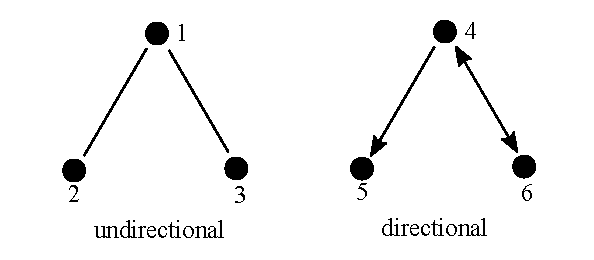
\includegraphics[width = .5\linewidth]{img/dir_undir_network.pdf}
    \caption{Schematic of directed versus undirected networks.}
    \label{fig:dir_undir}
\end{figure}

A network is weighted, when the connections are assigned weights.

The approach we choose is describing the system with a weighted directed network. Suggestively, we say that $u$ is \textbf{following} $v$, if $u$ is connected to $v$. A vertex $v$ is then influenced only by the vertices it is following. The weight that is assigned to the connection is called the \textbf{trust} of $u$ in $v$.\\
The trust measures how much $u$ is influenced by $v$, and is a dynamic variable.

\subsection{Opinion Evolution and Confidence}
The opinion of a vertex evolves in a similar way as is described by Hegselmann and Krause\cite{review_od}. A vertex adheres to his opinion with a certain \textit{degree}. We call this degree the \textbf{confidence} that $u$ has in its own opinion, $c(u)$. The evolution of the opinion is then calculated as a weighted mean over the opinions of the vertices that $u$ follows. The confidence induces a latency in the change of opinion; a high confidence means that the opinion change is smaller. This is explained in more detail in Section \ref{sec:implementation}.\\

For a more realistic model, an alternative interpretation of a vertex' opinion is the opinion the vertex perceives to be the consensus. In a filter bubble, an agent believes that everybody holds a similar opinion to his own.

\subsection{Following and Unfollowing -- Filter Bubbles}

The connections of the network are dynamically updated.\\
A vertex $u$ can sever a connection to $v$, as well as create a new one with $v'$. We say $u$ \textbf{unfollows} $v$ and \textbf{follows} $v'$.\\
We model the following and unfollowing process to be stochastical.
The probability of $u$ unfollowing $v$ is dependent on the trust that $u$ has in $v$. If the trust is low, unfollowing becomes more likely.\\
The probability of $u$ following $v'$ is modeled to be dependent on the opinion difference between the two vertices.\\

This step is where filter bubbles can be implemented and is therefore the 'heart' of this model. By regarding the probability of $u$ following $v$ as the probability that the social media platform \textit{proposes} to $v$ to follow $u$, and this probability diminishes if their opinions are further apart, this can lead to a separation of opinions, where one group does not in any way communicate with the other. For a visualisation, see Figure \ref{fig:p_follow}.\\
This approach was chosen to model algorithms by social media, which analyse a user's opinions and personalise content and user suggestions to predominantly reflect these opinions.

%The dynamics of the system arise from the evolution and interaction of these parameters. The general form of the modelled evolution will be discussed here, while specific implementation will be discussed in Section \ref{sec:implementation}.\\
%We index the evolution by a parameter $t$, and also refer to it as time. Each time step, $\bm{W},\,\bm{c},\,\bm{o}$ are updated, according to the following rules:

%\begin{enumerate}[-]
    %\item The opinion $o_i$ of vertex $v_i$ evolves deterministically with a similar model as seen in other treatments of this problem\cite{review_od} (where 'confidence' is replaced with 'degree'), according to
    %$$ o_i(t+1) = (1-c_i) o_i(t) + c_i \frac{\sum_{j} w_{ij} o_j(t)}{\sum_{j} w_{ij}}.$$
    %Expressed in vector notation, this becomes
    %\begin{equation}\label{eq:opinion_evol}
        %\bm{o}(t+1) = (\bm{I} - \bm{C})\bm{o}(t) + \bm{C}\widetilde{\bm{W}}\bm{o}(t),
    %\end{equation} 
    %where $\bm{I}$ is the $N\times N$ identity matrix, $\bm{C} = \mathrm{diag}(\bm{c})$, and $\widetilde{\bm{W}}$ is the weight matrix with normalised rows.
    
    %\item Confidences are updated according to a function $f_\mathrm{confidence}$
    %\begin{equation}\label{eq:confidence_evol}
       % \bm{c}(t+1) = f_\mathrm{confidence}(\bm{W}(t), \bm{c}(t), \bm{o}(t)).
    %\end{equation}
    %Qualitatively, we choose this function in such a way, that a vertex gains confidence if its opinion is closer to the vertices he follows. This gives rise to acceleration and deceleration in the changes of opinion.
    
    %\item The weight matrix is updated according to some function $f_\mathrm{weight}$ of the confidences and opinions;
    %\begin{equation}\label{eq:weight_evol}
        %\bm{W}(t+1) = f_\mathrm{weight}(\bm{W}(t), \bm{c}(t), \bm{o}(t)).
    %\end{equation}
    %Often this is chosen in such a way, that a vertex values connections to vertices who hold similar opinions higher.
    
    %\item A vertex can sever a connection ('unfollow') or create one ('follow'). This process is modeled to be stochastic. A vertex $v_i$ will unfollow a vertex $v_j$ with a (uniform) probability $p_\mathrm{unfollow}$, and follow it with probability $p_\mathrm{follow}$. In general, we choose these probabilities to be functions of the opinions the vertices hold, as well as the previously existing bond strength;
    %\begin{equation}\label{eq:prob_f_uf}
       % p_\mathrm{unfollow} = p_\mathrm{unfollow}(\bm{W}, \bm{o}),\quad p_\mathrm{follow} = p_\mathrm{follow}(\bm{o}).
    %\end{equation}
    %This step is where filter bubbles can be implemented and is therefore the 'heart' of this model. By regarding $p_\mathrm{follow}$ as the probability that the social media platform proposes to $v_i$ to follow $v_j$, and this probability diminishes if $o_i$ and $o_j$ are farther apart, this can lead to a separation of opinions, where one group does not in any way communicate with the other. For a visualisation, see Figure \ref{fig:p_follow}.
    
%\end{enumerate}

\begin{figure}[H]
    \centering
    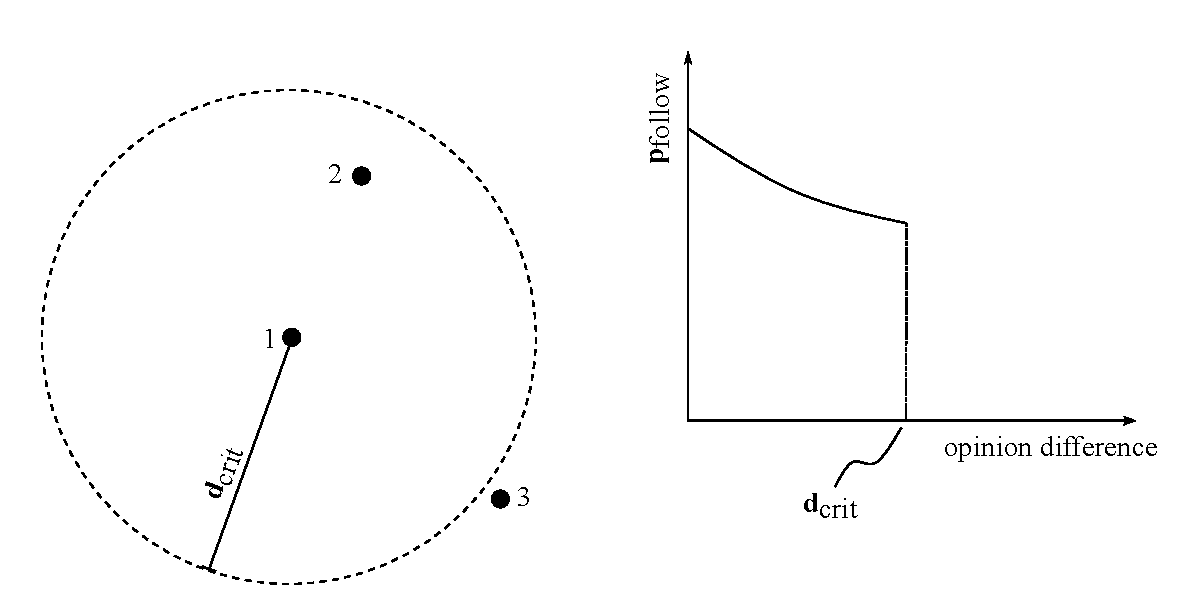
\includegraphics[width = .6\linewidth]{img/p_follow_visual.pdf}
    
    \caption{Three vertices with their respective distances visualising the opinion difference. A following probability $p_\mathrm{follow}$ which depends on the opinion difference between the vertices can result in filter bubbles. In this case, vertex 1 cannot be influenced by 3, since the probability to follow 3 is 0.}
    \label{fig:p_follow}
\end{figure}

\section{Implementation}\label{sec:implementation}
\subsection{Initial state}
Our network \((V, A)\) with the set of vertices \(V\) and set of edges \(A\) will be represented as an adjacency list.\par
In the initial state our network has no connections. By running the simulation for a while, the network will naturally build connections between mostly like-minded agents. This way we do not have to make initial artificial random connections which may be relatively unrealistic.\par
All our functions, namely opinion, trust and confidence, map to \([0,1]\) for reason of simplicity. They are concretely implemented as follows.
\subsubsection{Opinion}
\[o:V\rightarrow[0,1]\]
Each vertex will have an opinion value.\par
In our simulation we give uniformly random initial opinions but one could easily do it with an other distribution or give deterministic values.
\subsubsection{Trust}
\[w:A\rightarrow[0,1]\]
In the adjacency list, each vertex will have a set of vertices it follows. We will store a trust value for each of these vertices. If a vertex \(u\) is not connected to another vertex \(v\), i.e. \((u,v)\notin A\), we implicitly assume the value to be 0.\par
If a new connection from vertex \(u\) to \(v\) is built, the trust value will get initialized according to
\[w(u,v)\leftarrow \frac{1}{\max \{1, \deg^+(u)\}}\]
where \(\deg^+(u)\) is the number of vertices \(u\) follows (including the new one).

\subsubsection{Confidence}
\[c:V\rightarrow[0,1]\]
Each vertex will have a confidence value.\par
These values will not change over time. They are initialized randomly over a truncated normal distribution with bounds \(a=0.01,b=0.99\) and different values for the mean \(\mu\) and standard deviation \(\sigma\).

\subsection{Updating the network}
Our network will change over time. In the simulation we iterate over a defined number of time steps. Therefore we need to update our functions (opinion and trust) and the connections between agents in each time step of our simulation. The next sections describe how this is implemented.

\subsubsection{Updating opinion}
The opinion of a vertex \(u\) is updated as follows.
\[o(u)\leftarrow c(u)\cdot o(u) + (1-c(u))\cdot\overbrace{\sum\limits_{(u,v)\in A}\left(w(u,v)\cdot o(v)\right)}^{\textrm{other opinions}}\]
Firstly, we determine how opinions of other agents can influence a certain agent \(u\). The only opinions that the agent \(u\) considers are the opinions of those it follows. The vertex is more heavily influenced by vertices it trusts more. Therefore, we weight each opinion by the respective trust. Then, we take the weighted mean of opinions.\par
Secondly, we also take the opinion of \(u\) itself into account. This is done by multiplying the opinion of \(u\) by its confidence. Then we add to this the weighted sum of the other opinions multiplied by one minus the confidence (susceptibility). This means that, the higher the confidence of \(u\), the more it takes its own opinion into account and ignores the opinion of the ones it follows.

\subsubsection{Updating trust}
For each vertex \(u\) we update the trust in a vertex \(v\) it follows according to
\[w(u,v)\leftarrow w(u,v) + (1-\alpha)\cdot \left(c(v)-|o(u)-o(v)|\right)\] for \(0<\alpha<1\). We call \(\alpha\) the \textbf{trust stability}. The higher the trust stability, the slower the trust values change.\par
How the trust of \(u\) in \(v\) gets changed is dependent on the confidence of \(v\) and the opinion difference between the two agents. The more confident \(v\) is the more trust it will get from its followers, e.g. \(u\). But the higher the opinion difference is the less trust \(u\) will have in \(v\).\par
Furthermore, we normalize the trust values of each set of neighbours. We do this because we want to do weighted sums with the trust values of a vertex (see Updating opinion).

\subsubsection{Updating follower connections}\label{updatingfollower}
In this section we change the actual structure of the network.\par
In each time step we update the vertices a vertex follows. This is done for each vertex \(u\) by the following procedure.\par
Firstly, we do the unfollowing. This is simply done by iterating through all agents \(v\) which \(u\) follows and unfollowing them with a certain probability \[\Pr [u\ \mathrm{unfollows}\ v]=\exp (-\beta_u\cdot w(u,v)),\ \beta_u\in\mathbb{R}_{\geq0}.\]\par
Secondly, we build some new connections. We define an upper bound for how many new agents someone can follow in a time step. Then we iterate through all vertices \(v\) in a random order. If \(u\) does not yet follow \(v\) then \(u\) will follow it with a certain probability \[\Pr [u\ \mathrm{follows}\ v]=\exp (-\beta_f\cdot |o(v)-o(u)|),\ \beta_f\in\mathbb{R}_{\geq0}.\]\par
We see that \(\Pr [u\ \mathrm{follows}\ v]\) depends on the opinion difference between the two agents. This should represent the algorithm of any social network that recommends new people to a user. The idea is that we want users to find people which they find interesting.\par
The probability \(\Pr [u\ \mathrm{unfollows}\ v]\) is dependent on the trust that agent \(u\) has in \(v\). The higher the trust the lower the probability of unfollowing.

\section{Simulation Results and Discussion}
The goal of the following section is to investigate the results obtained by changing the basic parameters of the model. These are the values $\beta_u$ and $\beta_f$, which determine the probabilities for following and unfollowing, $confidence\_mean$ and $confidence\_std$, which determine the probability distribution of the confidence and $trust\_stability$, which affects how fast the trust values change.

\subsection{Initial Setup}
As the initial setup the basic parameters for the model are set as follows:

\begin{lstlisting}[language=Python]
bu = 20
bf = 20
confidence_mean = 0.9
confidence_std = 0.1
trust_stability = 0.99
\end{lstlisting}
The initial opinions are uniformly distributed over the interval $[0,1]$.\\
This initial setup is used for all further investigations of the model. Running the simulation on the initial setup results in two filter bubbles.

\begin{figure}[H]
    %\centering
    \begin{subfigure}[t]{0.5\textwidth}
    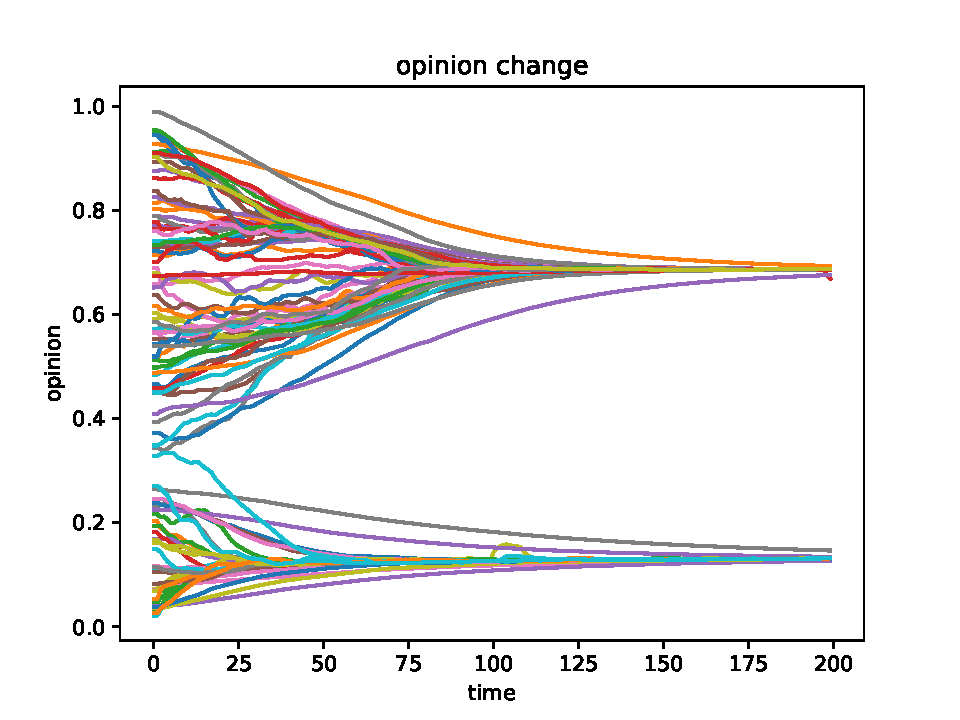
\includegraphics[width = \linewidth]{img/initial_setup_opinions.pdf}
    \caption{Opinions ending up in two filter bubbles}\label{sfig:opinit}
    \end{subfigure}
    ~
    \begin{subfigure}[t]{0.5\textwidth}
    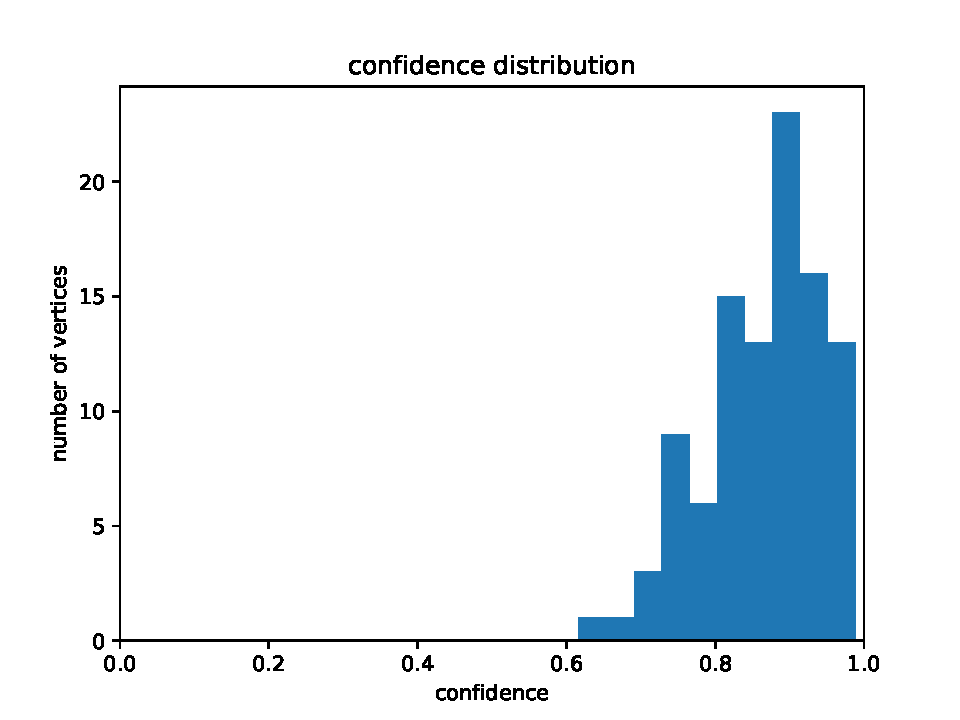
\includegraphics[width = \linewidth]{img/initial_setup_confidence.pdf}
    \caption{Distribution of confidence}\label{sfig:confdist_init}
    \end{subfigure}
    \caption{In (\ref{sfig:opinit}), the changes of opinions, resulting in two filter bubbles at $0.65$ and $0.18$, are plotted over time. (\ref{sfig:confdist_init}) displays the distribution of confidence.}\label{sfig:init}
\end{figure}
Different simulations with the same initial model differ only in the opinions around which the filter bubbles build up.

\subsection{Influence of $p\_follow$ and $p\_unfollow$}

The amount of filter bubbles at the end of a simulation is highly dependent on $p\_follow$ and $p\_unfollow$. In the model, these two values depend on the parameters $\beta_f$ and $\beta_u$. How these two probabilities are calculated is described in subsection \ref{updatingfollower}.\\
Increasing $\beta_u$ means that the the probability to unfollow some other vertex gets smaller if the trust in this vertex has not changed. In other words the trust in another vertex has to decrease in order to unfollow this vertex if $\beta_u$ has increased.\\
Increasing $\beta_f$ decreases the probability to follow some other vertex if the opinion difference between the two vertices has not changed. In other words, the opinion difference between two vertices has to get smaller to accept a follow suggestion if $\beta_f$ has increased.

\subsubsection{Varying $\beta_u$}

\begin{figure}[H]
    %\centering
    \begin{subfigure}[t]{0.5\textwidth}
    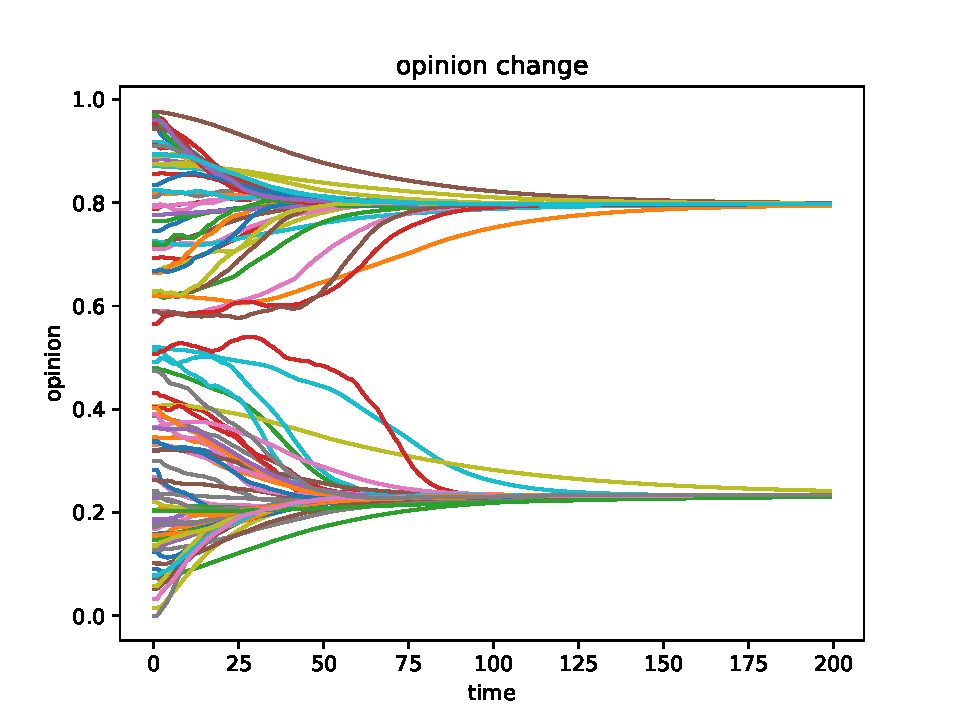
\includegraphics[width = \linewidth]{img/bu_high_1.pdf}
    \caption{$\beta_u=80$}\label{sfig:buhigh1}
    \end{subfigure}
    ~
    \begin{subfigure}[t]{0.5\textwidth}
    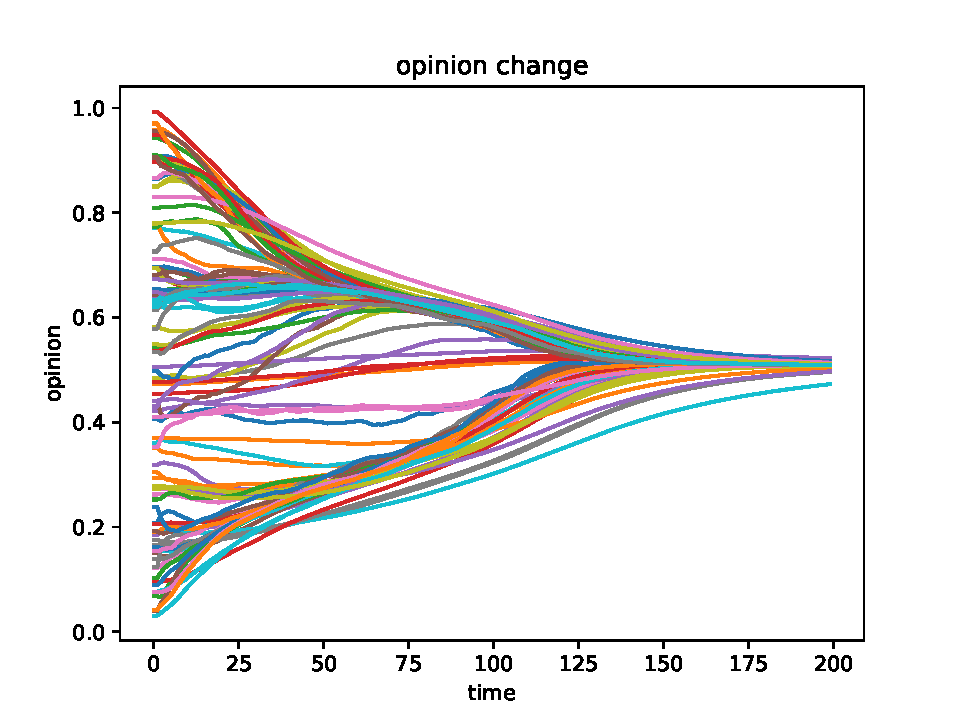
\includegraphics[width = \linewidth]{img/bu_high_2.pdf}
    \caption{$\beta_u=200$}\label{sfig:buhigh2}
    \end{subfigure}
    \caption{Increasing $\beta_u$ to 80 (\ref{sfig:buhigh1}) respectively 200 (\ref{sfig:buhigh2}) while leaving $\beta_f$ at 20.}\label{sfig:buhigh}
\end{figure}
Increasing $\beta_u$ while leaving $\beta_f$ at a value of 20 leads to the fact that it is less likely to unfollow another vertex. Hence the opinions settle in two respectively one filter bubble. Since one agent is influenced by every other agent it follows, this result makes perfect sense. After some time every agent follows every other vertex whose opinion is in some range. In this case the range depends on the value of $\beta_u$. Increasing $\beta_u$ also increases this range. At the end all agents in one range agree to the same opinion and therefore a filter bubble comes into existence. For $\beta_u=80$ there are two such ranges and for $\beta_u=200$ there is only one.

\subsubsection{Varying $\beta_f$}

\begin{figure}[H]
    %\centering
    \begin{subfigure}[t]{0.5\textwidth}
    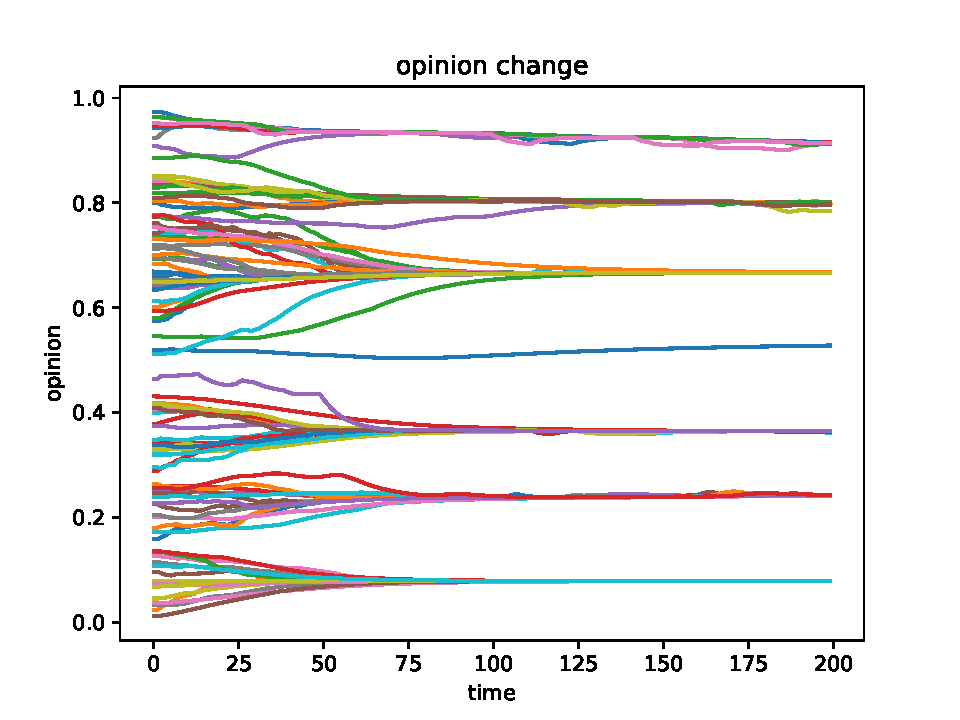
\includegraphics[width = \linewidth]{img/bf_high_1.pdf}
    \caption{$\beta_f=80$}\label{sfig:bfhigh1}
    \end{subfigure}
    ~
    \begin{subfigure}[t]{0.5\textwidth}
    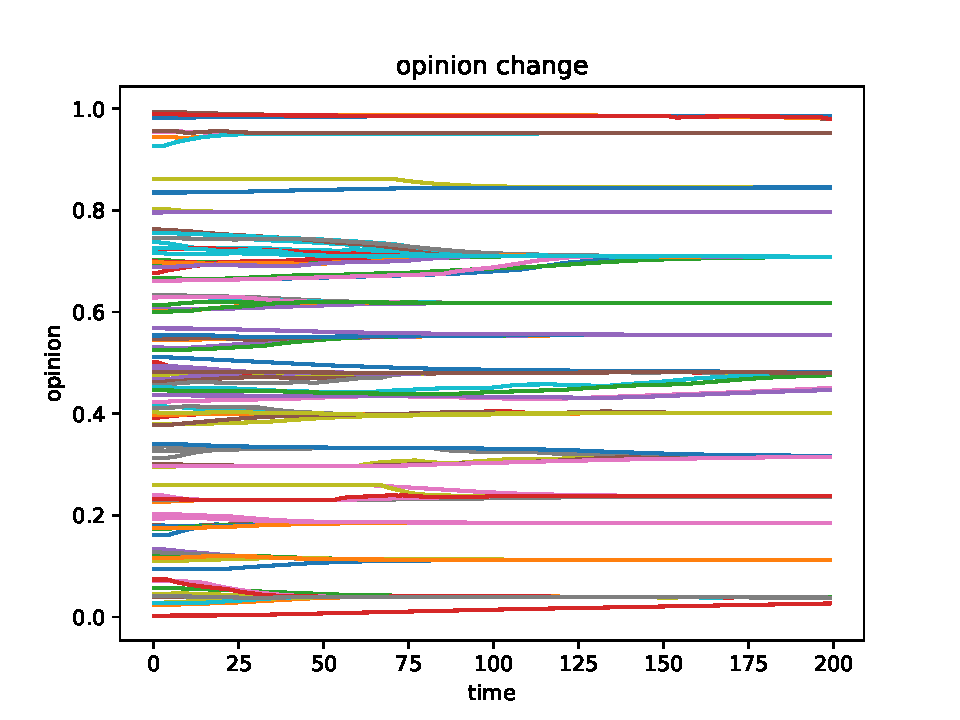
\includegraphics[width = \linewidth]{img/bf_high_2.pdf}
    \caption{$\beta_f=200$}\label{sfig:bfhigh2}
    \end{subfigure}
    \caption{Increasing $\beta_f$ to 80 (\ref{sfig:bfhigh1}) respectively 200 (\ref{sfig:bfhigh2}) while leaving $\beta_u$ at 20.}\label{sfig:bfhigh}
\end{figure}
Increasing $\beta_f$ leads to a much lesser tolerance of the agents, meaning that the opinion difference between an agent and a suggested other agent has to be much smaller for the agent to accept the suggestion. In the end, this as well leads to ranges in which it is possible for agents to follow each other. However, in contrast to $\beta_u$, $\beta_f$ is direct proportional to the amount of ranges. In conclusion, increasing $\beta_f$ leads to more filter bubbles.\\
If $\beta_f$ is too large, the agents tend to not accept any suggestions and therefore keeping their initial opinion.
% habe influence of the confidence distribution in den appendix getan

\subsection{Trust stability}

\begin{figure}[H]
    %\centering
    \begin{subfigure}[t]{0.5\textwidth}
    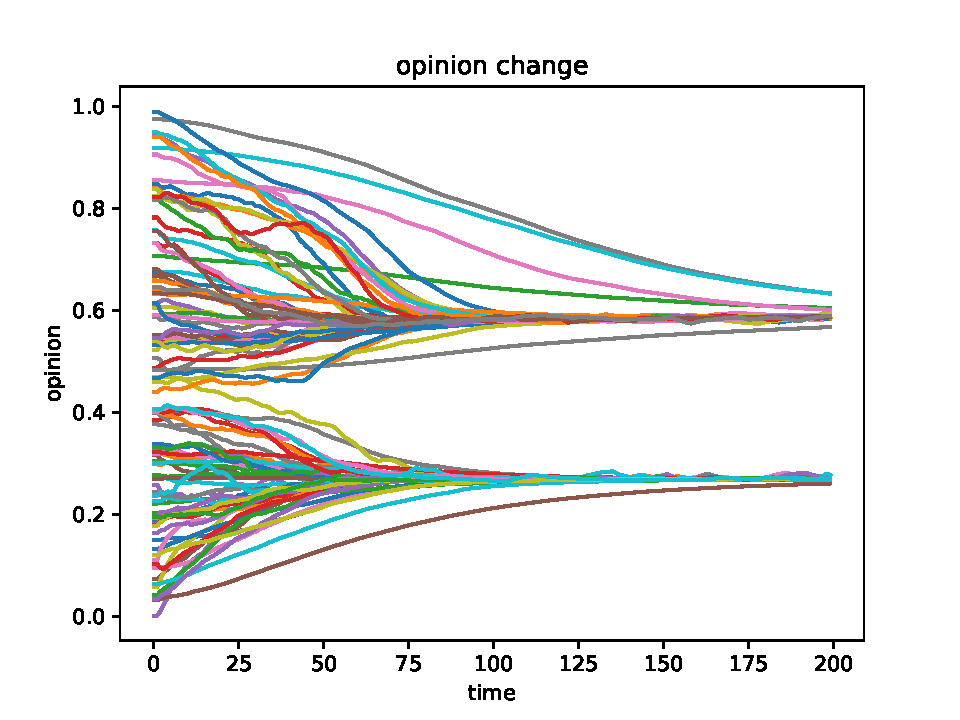
\includegraphics[width = \linewidth]{img/trust_stability_1.pdf}
    \caption{Changes in opinion for $trust\_stability=0.5$}\label{sfig:trust1}
    \end{subfigure}
    ~
    \begin{subfigure}[t]{0.5\textwidth}
    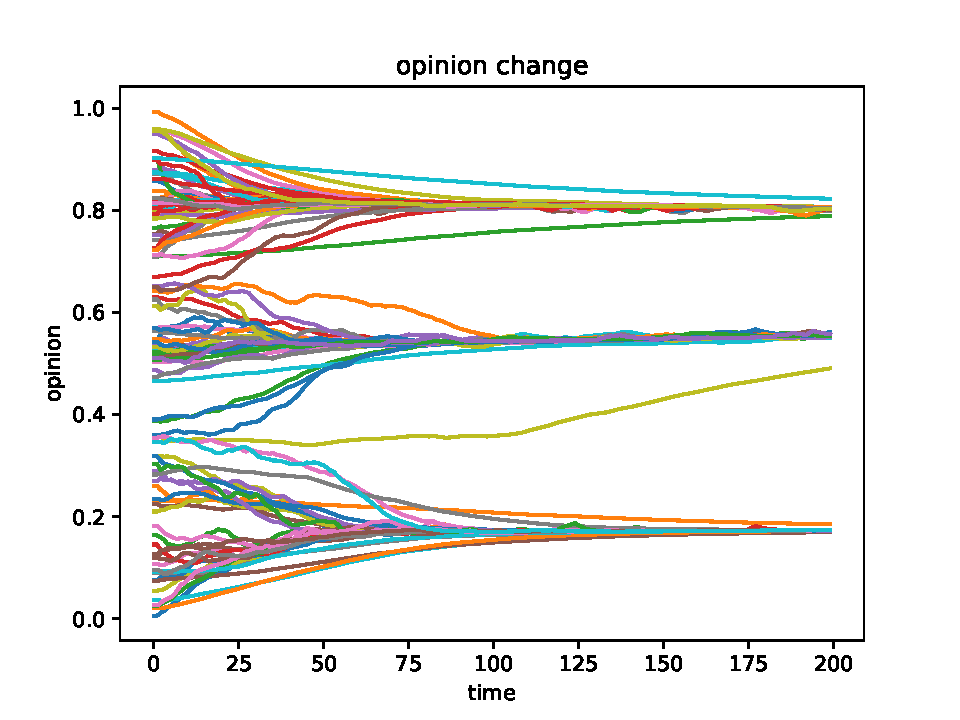
\includegraphics[width = \linewidth]{img/trust_stability_2.pdf}
    \caption{Changes in opinion for $trust\_stability=0.5$}\label{sfig:trust2}
    \end{subfigure}
    \caption{Changing the value of $trust\_stability$ can cause slower convergence of opinions (\ref{sfig:trust1}) or it can even increase the amount of filter bubbles (\ref{sfig:trust2}).}\label{sfig:trust}
\end{figure}
Reducing the $trust\_stability$ can have two effects on the opinion formation. In general the opinions converge slower. However, it is also possible that the amount of filter bubbles increases. That is because if the trust stability is smaller, the trust values for the different agents change more.

\subsection{Merging of Opinion Bubbles}

We can observe critical behaviour for the merging of two opinion strands. When initialising, opinions are grouped into two strands, separated by a certain number (separation). The probability of the strands to merge is recorded for different separations and different coefficients $\beta_f$, determining the following probability
$$\Pr[u\text{ follows }v] = \exp(-\beta_f|o(u) - o(v)|).$$
Results are shown in Figure \ref{fig:convProb}. We observe that there is a critical strand separation, at which the probability of the strands to merge falls from 1 to 0 quickly. For larger $\beta_f$, this critical separation is lower. For $\beta_f = 5$, the merging probability is fitted with a Fermi-Dirac distribution function $f(s) = \frac{1}{\exp((s-a)/b) + 1}$. The fitted parameters are
$$a_\mathrm{fit} = 0.711 \pm 0.007,\quad b_\mathrm{fit} = 0.048 \pm 0.007.$$

In the "thermodynamic" limit, the dependence might be better described by a function similar to percolation models,
$$\Pr[\text{merging of strands}] \propto 1 - |s - s_\mathrm{crit}|^\gamma,\quad s > s_\mathrm{crit},$$
where $s$ is the strand separation, and $s_\mathrm{crit}$ is a critical separation. A thorough investigation of such a relation is limited by computation times.

\begin{figure}[H]
    \centering %removed for horizontal alignment
    \begin{subfigure}[t]{.6\textwidth}
    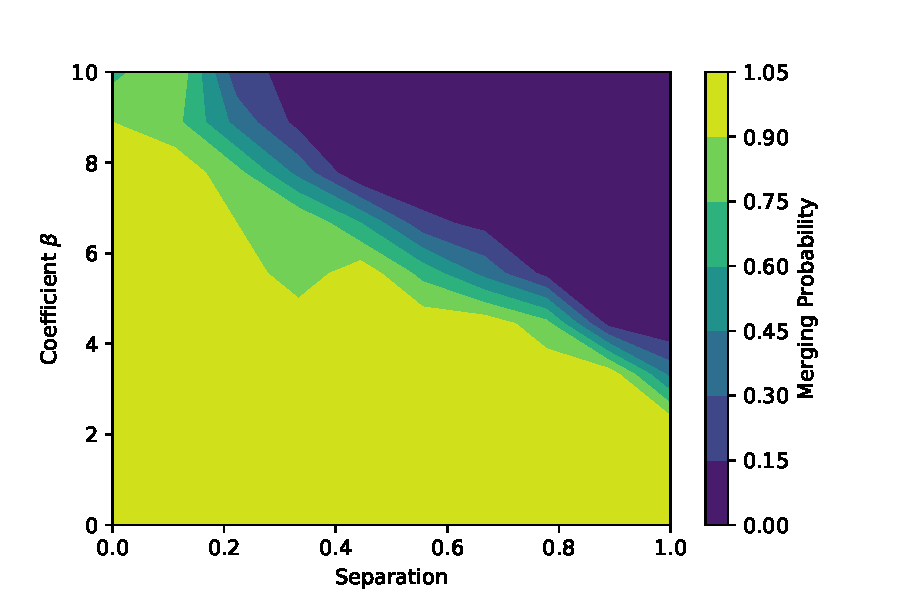
\includegraphics[width = \linewidth]{img/contourtest.pdf}
    \caption{The merging probability for different following probabilities, characterised by $\beta_f$.}\label{sfig:2dconv}
    \end{subfigure}
    ~
    \begin{subfigure}[t]{.6\textwidth}
    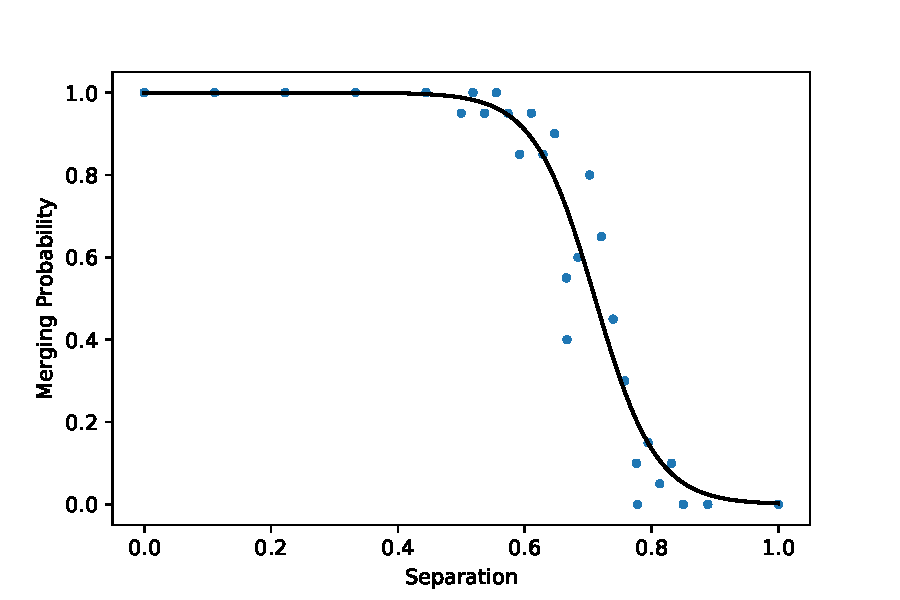
\includegraphics[width = \linewidth]{img/beta5.pdf}
    \caption{Fitted merging probability for $\beta_f = 5$.}\label{sfig:fitconv}
    \end{subfigure}
    \caption{The probability of two strands to merge for different initial strand separations. In \ref{sfig:2dconv}, the probability is plotted for different $\beta_f$ coefficients. In \ref{sfig:fitconv}, the curve is shown in more detail for $\beta_f = 5$ and fitted with a function of the form $f(s) = \frac{1}{\exp((s-a)/b) + 1}$.}
    \label{fig:convProb}
\end{figure}

\section{Summary and Outlook}

We have implemented a relatively simple agent-based model to study filter bubbles in opinion formation, motivated by a social media phenomenon.\\

We were able to extract qualitative statements about the effect of various parameters on the formation of filter bubbles.\\
Notably, we studied the effect of different following and unfollowing probabilities. We found that for low following probabilities for large opinion differences, the formation of filter bubbles becomes more likely. This is because communication between vertices of different opinions becomes unlikely. A high unfollowing probability for low trust also results in formation of bubbles, as a vertex is more likely to unfollow a vertex it disagrees with.\\
By varying model parameters such as trust stability and confidence, we were able to manipulate the convergence rate of filter bubbles.\\

We observed behaviour for the merging of different opinion bubbles, and found that there is a region critical opinion separation, where the merging probability falls sharply from 1 to 0. This is reminiscent of basic percolation behaviour, and could be studied in more detail.\\

It would also be interesting to consider different network structures, where a vertex does not have the opportunity to in principle communicate with any other vertex. Our approach was chosen to model social media, however, geographic separation, age, and other factors also have an effect on the connections in realistic social media networks. If other network structures were to be considered, we would expect to see more complex behaviour.\\

It is a possibility to use real-world data and study, which aspects of the dynamics are captured by our model. While it is unlikely that the model is able to realistically describe the system, it might give valuable insights, both into social media dynamics as well as improvement of the model.

%\newpage
\begin{thebibliography}{9}
    \bibitem{quote} Kevin J. Delaney (February 21, 2017). "Filter bubbles are a serious problem with news, says Bill Gates". Quartz. Retrieved 15 November 2019.
    
    \bibitem{wikiquote} Wikipedia, Wikimedia Foundation. Last accessed 15 November 2019.\\\texttt{en.wikipedia.org/wiki/Filter\_bubble}
    
    \bibitem{USBubble}
    Medium, A Medium Corporation. Last accessed 20 November 2019.\\ \texttt{medium.com/@willrinehart/the-election-of-2016-and-the-\\filter-bubble-thesis-in-2017-51cd7520ed7}
    
    \bibitem{review_od}
    Hegselmann, R., Krause, U., JASS \textbf{5}, 3, 2002,\\
    \textit{Opinion Dynamics and Bounded Confidence}
    
\end{thebibliography}

\newpage

\appendix
%\section{Appendix}

%%%%%%%%%%%%%%%%%%%%%%%%%%%%%%%%%%%%%%%

\section{Declaration of Originality}
\begin{center}

\includegraphics[scale = 0.8]{doc/latex/declaration-originality.pdf}
\end{center}

%
\includepdf[]{doc/latex/declaration-originality.pdf}
% IMPORTANT
% you MUST include the ETH declaration of originality here; it is available for download on the course website or at http://www.ethz.ch/faculty/exams/plagiarism/index_EN; it can be printed as pdf and should be filled out in handwriting

\section{Further Analysis}
\subsection{Influence of the confidence distribution}
In the initial setup the confidence values get initialized randomly over a truncated normal distribution with the mean $\mu=0.9$ and standard deviation $\sigma=0.1$.\\
This section determines the influence of changing $\mu$ and $\sigma$ for this distribution.
\subsubsection{Changing $\mu$}

\begin{figure}[H]
    %\centering
    \begin{subfigure}[t]{0.5\textwidth}
    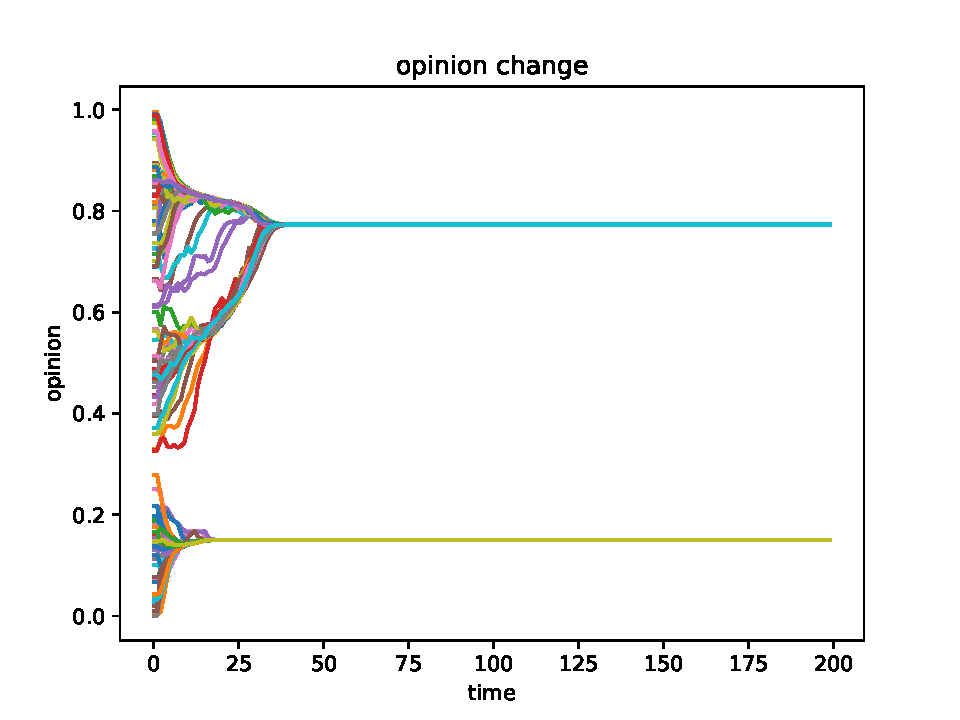
\includegraphics[width = \linewidth]{img/mu_3.pdf}
    \caption{Changes in opinion for $\mu=0.3$}\label{sfig:mu3}
    \end{subfigure}
    ~
    \begin{subfigure}[t]{0.5\textwidth}
    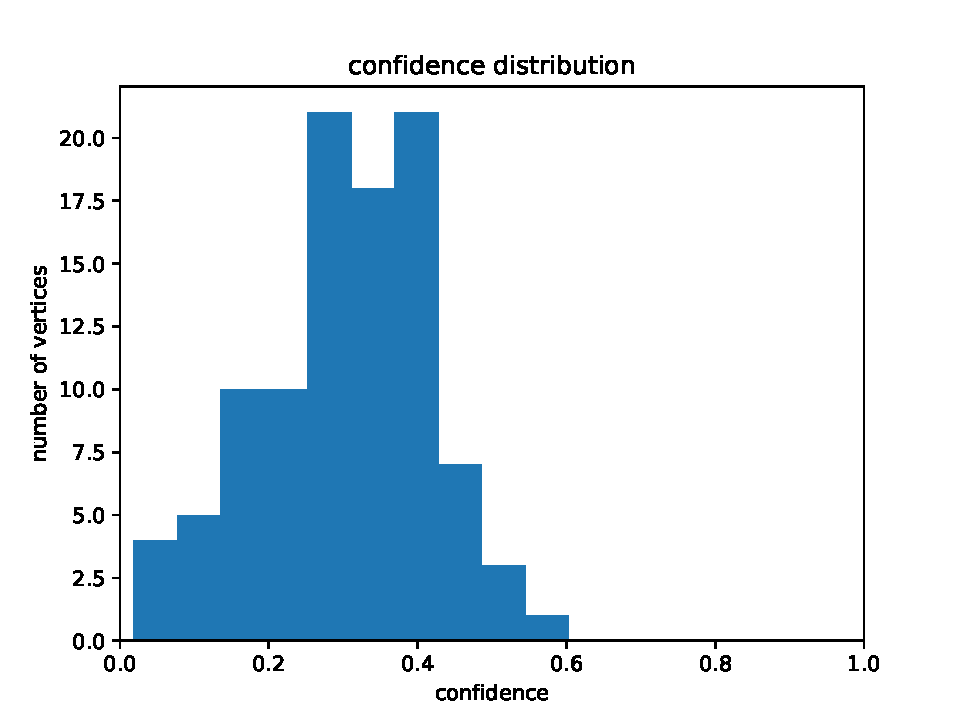
\includegraphics[width = \linewidth]{img/mu_33.pdf}
    \caption{Confidence distribution for $\mu=0.3$}\label{sfig:mu33}
    \end{subfigure}
    \caption{Changing the value of $\mu$ from 0.9 to 0.3}\label{sfig:mu1}
\end{figure}
Changing $\mu$ from 0.9 to 0.3 leads to lower confidence of the agents. And therefore the agents change their opinions faster, the opinions converge faster and the filter bubbles get established faster.

\subsubsection{Changing $\sigma$}

\begin{figure}[H]
    %\centering
    \begin{subfigure}[t]{0.5\textwidth}
    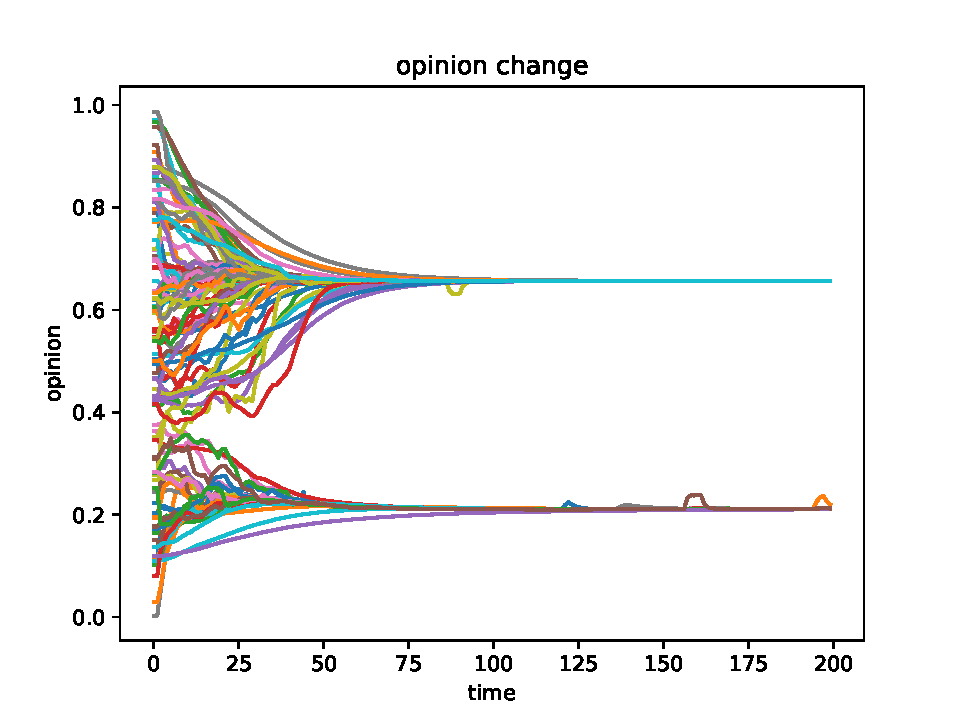
\includegraphics[width = \linewidth]{img/sigma_7.pdf}
    \caption{Changes in opinion for $\sigma=0.7$}\label{sfig:sig7}
    \end{subfigure}
    ~
    \begin{subfigure}[t]{0.5\textwidth}
    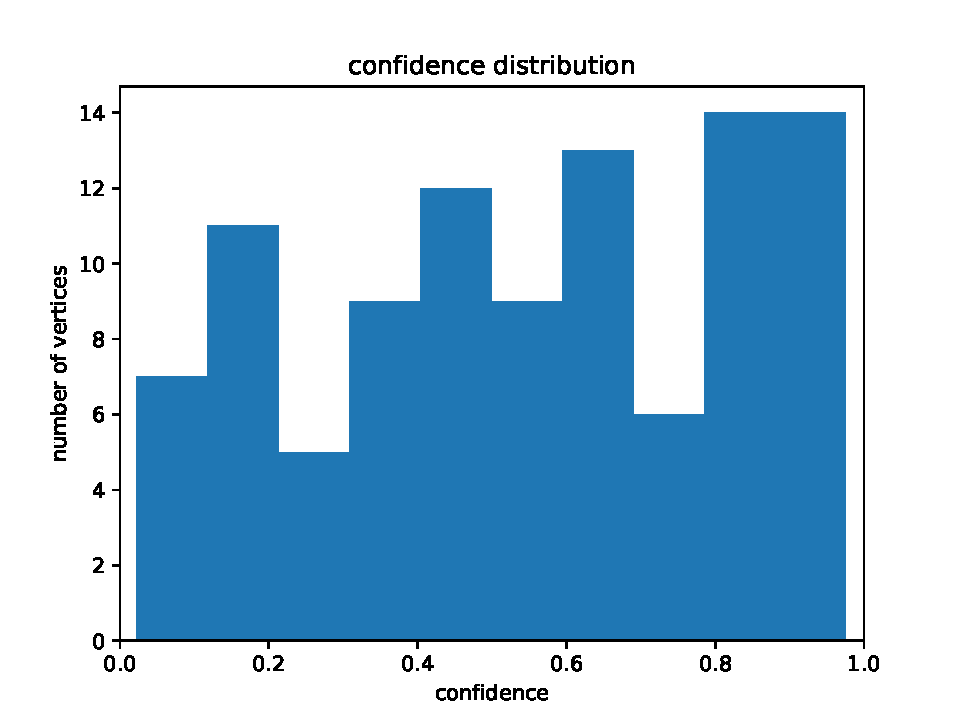
\includegraphics[width = \linewidth]{img/sigma_77.pdf}
    \caption{Confidence distribution for $\sigma=0.7$}\label{sfig:sig77}
    \end{subfigure}
    \caption{Changing the value of $\sigma$ from 0.1 to 0.7}\label{sfig:sig1}
\end{figure}

Changing the value of $\sigma$ while keeping the value of $\mu=0.9$ influences the speed of convergence. Because the higher $\sigma$, the more agents there are, which have little confidence. Furthermore, these agents change their opinion faster and therefore support a faster convergence of opinions.



\end{document}  



 
